
\documentclass[12pt]{article}
\usepackage[T1]{fontenc}
\usepackage[utf8]{inputenc}
\usepackage{amsmath}
\usepackage{microtype}
\usepackage{listings}
\setlength{\parindent}{0pt}
\usepackage{fancyvrb}
\usepackage{enumerate}
\usepackage{array}
\usepackage[breaklinks=true,linktocpage,hidelinks]{hyperref}
\usepackage[letterpaper]{geometry}
\usepackage{url}
\usepackage{graphicx}
\usepackage{fullpage}

\usepackage{pgfplots}
\usepackage{pgfplotstable}
\usepackage{tikz}

\usepackage{fancyhdr}
\usepackage{fancybox}
\usepackage{multicol}
\usepackage{xcolor}
\usepackage{adjustbox}

\pgfplotsset{compat=newest}
\usetikzlibrary{shapes,backgrounds,arrows}
\usepgfplotslibrary{external} 

\definecolor{brewcol1}{RGB}{166,206,227}
\definecolor{brewcol2}{RGB}{31,120,180}
\definecolor{brewcol3}{RGB}{178,223,138}
\definecolor{brewcol4}{RGB}{51,160,44}
\definecolor{brewcol5}{RGB}{251,154,153}
\definecolor{brewcol6}{RGB}{227,26,28}
\definecolor{brewcol7}{RGB}{237,179,1}
\definecolor{brewcol8}{RGB}{202,178,214}
\definecolor{brewcol9}{RGB}{206,27,1}

\geometry{hmargin=1.87cm, vmargin=1.87cm}
\bibliographystyle{siam}

\DeclareTextFontCommand{\helvetica}{\fontfamily{phv}\selectfont\small}


\begin{document}

\clearpage\thispagestyle{empty}
\begin{center}
\textbf{Difficult transition for sugar maple in Boreal forest under climate change? \\
Impact of alternative stable states on Sugar maple migration.}
\vskip 2em
Research proposal
\vskip 1em
Master in Wildlife management
\vfill
By
\vfill
Steve Vissault 
\vfill 
For
\vfill
\textbf{Richard Cloutier}, Pr.\\
Director of the program committee
\vskip 2em
\textbf{Dominique Arsenault}, Pr.\\
President of the jury
\vskip 2em
\textbf{Matt Talluto}, PhD\\
Research Co-director
\vskip 2em
\textbf{Dominique Gravel}, Pr.\\
Research Director
\vfill
\vfill
Université du Québec à Rimouski\\
\today

\end{center}

\newpage
\setcounter{page}{1}

\section{Introduction}

\textbf{Context.} Sugar maple (\textit{Acer saccharum}) is a widespread and
abundant tree in north-eastern North America.
\cite{Graignic2013,Messaoud2007,Kellman2004,Barras1998}. Predicting shifts in
the range of Sugar maple is an important challenge because this species is
highly desirable by hardwood and maple syrup producers, two large economic
sectors in Quebec. This species is dominating the northern temperate forest
especially along the boreal-temperate forests ecotone at its northern range
limit \cite{Barras1998}. Some species mostly representative of northern
forest ecosystems are forecast to expand their distribution broadly towards
the north \cite{Sciences2014,Iverson2002}. According to McKenney (2007)
\cite{Sciences2014}, Sugar maple is one of those species expected to move
closed to the Ungava bay which appear highly improbable. In fact, Sugar maple
predictions are built on species distribution models based only on climatic
conditions, though Sugar maple regeneration depends both on macro conditions
(\textit{i.e.} regional climate) and micro conditions (\textit{i.e.} soil and
microtopography) \cite{Graignic2013,Lafleur2010}. Thus, the expansion of Sugar
maple and its temperate species community is difficult to predict because
micro conditions can mitigate macro conditions such as global warming
\cite{DeFrenne2013}.\\

Species respond differently to the soil conditions, and the soil
properties found in boreal forests are different from those in temperate
forest \cite{Lafleur2010,Barras1998,Goldblum2010,Demers1998}. Conifer forests
generally contain deep and poorly-decomposed litter layers, while those of
northern hardwood forests are thinner but covered by a tough superficial leaf
mat \cite{Barras1998}. In boreal forest, the temperature is colder and the
snow melts later, the soil is wetter and the litter is more acidic and fibrous
\cite{Lafleur2010,Goldblum2010}. Soil acidification causes a reduction in
the cation exchange capacity and subsequently decreases availability of some
nutrients such as calcium \cite{Moore2008}. Sugar maple seedlings have been
recognized to be particularly sensitive to waterlogged conditions and soil nutrient
content \cite{Moore2008,Lafleur2010,Cleavitt2011}. These properties of
coniferous forest soils could hinder the local establishment of species
associated with alkaline soils or unable to withstand waterlogged conditions
\cite{Lafleur2010}. Under these latter conditions, tree species migration is
likely to be restricted or delayed \cite{Lafleur2010}. Thus even if the
regional climate conditions are favorable, the micro conditions found in the
boreal forest could slow the seedling establishment of these temperate
species \cite{Kellman2004,Moore2008,Barras1998,Messier2011}. Then the
temperate forest including Sugar maple could be unable to migrate in
boreal forests as a result of local plant-soil feedbacks
\cite{McCarthyNeumann2012}. To study the expansion of Sugar maple, the ecotone
dynamic can be conceptualized as two dominant communities:
the boreal community and the temperate community including Sugar maple. The
landscape might be structured as a patchy mosaic where micro
conditions are driving the spatial occurrences of boreal and temperate
community species despite a regional climate favourable to temperate species
\cite{Goldblum2010,Fisichelli2013}. In this case, these forest communities are
two alternative stable states, \textit{i.e.} contrasted states occurring in the
same climate conditions \cite{scheffer2009critical}. This situation generate a
tension between the boreal and temperate forest meaning that modification of
micro conditions (i.e mainly soil conditions) can produce abrupt shifts in
community composition in the boreal-temperate forest ecotone.\\

\textbf{Objectives.} The main objective of this project is to investigate the
transition between the boreal and temperate forests under different climate
change scenarios. In this context, we will test two different hypotheses:
($H_1$) Alternative stable states are occurring in the boreal-temperate forests
ecotone, and ($H_2$) Time lags in the response to climate change will be larger
in areas where alternative stable states are occurring. In order to achieve the
general objective and test these hypotheses, we will (1) develop a climate-dependent
state-transition model (STM) representing the dynamics of the
boreal and temperate communities at landscape scale; (2) investigate the
spatial structure of maple distribution through its temperate community; (3)
Study the occurrence of alternative stable states in the transitional zone;
and finally (4) run simulations of the temperate community species
distribution under different climate change scenarios. The first section of
this proposal reviews the context of the study. The first part of the review
presents the concept of alternative stable states and critical transitions in
forest ecosystem properties. The second part focuses on Sugar maple, its
associated community in the temperate biome, and a justification about why
alternative stable states are expected to occur at the boreal-temperate
forests ecotone. The last section of this document describes the model and
the methodology that we will employ to achieve the specific objectives.

\section{Review}

\begin{figure}[t]
\begin{center}
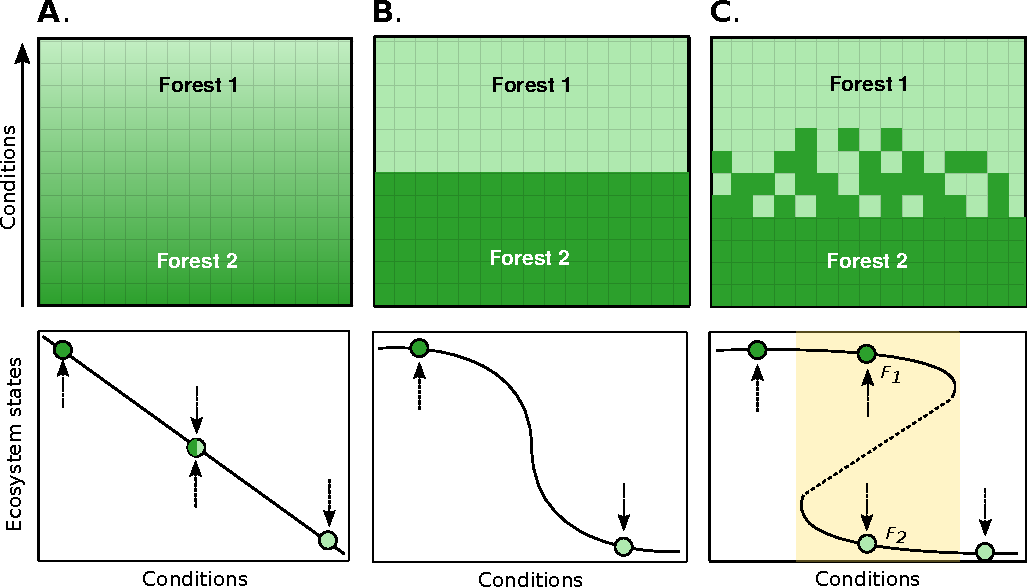
\includegraphics[width=0.8\textwidth]{fig/states.pdf}
\end{center}
\caption{Schematic representation of different ways in which the equilibrium
states from forest-forest system can vary over environmental gradients such as temperature, precipitation
or soil moisture. Three different responses are presented,
\textbf{(A)} gradual, \textbf{(B)} basic fold, \textbf{(C}) catastrophic fold.
The first line presents the stable ecosystem states
given a specific environmental condition. Arrows indicate the
direction the system moves if not at the equilibrium.
Solid lines represent stable states along the boreal-temperate
transition, and the dashed line (in yellow highlight) unstable equilibrium. This zone,
called hysteresis, is particularly unstable and small fluctuations in
environment conditions give rise to a contrasted state representing an
alternative stable states. ($F_1$ or $F_2$).
The second line illustrates a conceptualization of a transitional landscape
between the boreal (light green) and the nordic temperate forests (dark
green).}
\label{fig1}
\vspace{-1.25em}
\end{figure}


\textbf{Alternative stable states in forest ecosystems.} The idea that
alternative stable states may exist in community ecology emerged in the late
1960s \cite{Scheffer2001,Society2014a}. May (1977) highlights the fact than an
ecosystem can be seen as a dynamic system where communities possess several
different equilibrium points given a specific external conditions
\cite{May1977}. These equilibrium states are named alternative stable states.
Suppose that a forest ecosystem can be usefully characterized by a set of
dynamic state variables, with their relations to each other defined by a set
of external conditions. In the present context, a state is defined as a forest
species community given a time and a set of environmental conditions (e.g.
annual precipitation and annual temperature). Changes on this set of
environmental parameters can induce three different shapes of ecosystem
response: \textbf{(A)} gradual, \textbf{(B)} basic fold, \textbf{(C})
catastrophic fold \cite{Scheffer2001} (Figure \ref{fig1}, upper line).
Firstly, when a small environmental change occurs, forest ecosystems can
respond almost linearly, with no threshold leading to drastic changes in the
species community (Figure \ref{fig1}.a, upper line)
\cite{Scheffer2001,Scheffer2009}. In this case, forest ecosystems can be seen
as a continuum of states along the climate gradient
\cite{Scheffer2001,Scheffer2009,scheffer2009critical}. For instance, when the
annual precipitation increases slightly in a deciduous stand, the new local
condition gives rise to a new coniferous species establishment (e.g balsam
fir). This forest stand reaches a new state wherein the species community has
been smoothly changed. Secondly, such forest ecosystems are insensitive to
small changes in environmental conditions over certain ranges but respond
strongly when a threshold is reached \cite{scheffer2009critical}. For example,
species mortality can increase sharply when the water level of a lake is
rising permanently in response to changing hydrological conditions in the
drainage basin. The new condition abruptly changes the entire species
assemblage surrounding the lake. Hence, the response curve of the natural
system is not linear but lightly folded and these changes can drive the forest
ecosystem to a threshold and lead to major changes in the community (Figure
\ref{fig1} .b, upper line). Lastly, in some non-linear systems, the response
curve can be folded backwards and alternative stable states could occur
(Figure \ref{fig1} .c). When the system approaches a tipping point on the
folded upper branch, it cannot pass smoothly to the lower branch. Small
forcing on initial conditions of the state $F_1$ transfer the system
immediately into a different state $F_2$ (Figure \ref{fig1} .c). Hence, at
this point, the system is particularly sensitive to the initial conditions.
This point is called a bifurcation point and a small forcing on it can drive
the system into backward or forward shifts towards either alternative stable
states \cite{scheffer2009critical}. The main ingredient to creating
alternative stable states is positive feedbacks \cite{scheffer2009critical}.
One well known is facilitation in ecological succession (i.e. the idea that
pioneer species pave the way for later successional species) and this feedback
seems to be present in the the boreal-temperate forests studied
\cite{Barras1998,Society2014}. \\


\textbf{Natural system studied.} Many empirical and modelling studies have been
conducted on the transition between forest to non-forests (e.g. Boreal-Tundra)
\cite{Scheffer2012,Scheffer2001,Hirota2011,Messaoud2007} but little
attention has been given to evaluate the forest-forest ecotone
\cite{Goldblum2010,Graignic2013,Messaoud2007}. At landscape scales, transitions
between the temperate and boreal forests can be approached as a dynamical
system where each forest biome community is a stable state (Figure \ref{fig1},
lower line). There is no distinct boundary at the boreal-temperate ecotone;
instead a broad transition zone exists where stands of coniferous and
deciduous species co-occur at the regional scale
\cite{Goldblum2010,Fisichelli2013}. A macromosaic landscape can be observed
with either pure stands of northern temperate trees or boreal forest stands
\cite{Goldblum2010,Fisichelli2013}. In this study context, alternative stable
state theory could applied to the hardwood-boreal forest patchiness structure
often attributed to differences in soils, nutrient status and topographical
factors \cite{Society2014}. This segregated patch distribution could be
explained by the fact than microclimatic conditions can modulate establishment
of those forests \cite{DeFrenne2013}. Distribution of deciduous and boreal
forests within the ecotone is not determined by macroclimatic conditions, but
rather by local variation of substrate, drainage, physical soil properties,
and nutrient availability \cite{Goldblum2010,Society2014}. Boreal and hardwood
forests are dominated by trees with different physiognomy, which is expected
to produce distinctive litter and light micro-environments \cite{Barras1998}.
A positive feedback contributes to the maintenance of the community type if the
dominant tree species promotes conditions facilitating its own regeneration
\cite{Barras1998}. Frelich \textit{et al.}(1993) \cite{Society2014}
hypothesized that Sugar maple is subject to such a feedback. Hence, soil
conditions and role of dominant species in regeneration seems to act as main
feedbacks on the temperate forest establishment (Figure \ref{fig1}.c, upper
panel). Boreal soil can delay temperate species regeneration (negative
feedback) and, on other hand, temperate species establishment can enrich the
soil towards a better substrate to their own regeneration (positive feedback).
In this context, we expect to find forest stands dominated by either boreal
species or temperate species and with great sensitivity to initial conditions
(i.e. soil conditions, abundance of deciduous or coniferous
species in the forest stand). Thus, the soil condition and the role of
dominant species in boreal and temperate forests need to be investigate as main
drivers in shifts between alternative stable states
\cite{Kellman2004,Moore2008,DeFrenne2013,Barras1998}.

\section{Methods}

\begin{wrapfigure}{L}{0.45\textwidth}

\begin{center}
	
				\tikzstyle{noeud}=[circle,
				                  thick,
				                  minimum size = 1.5cm,
				                  inner sep =5pt,
				                  draw=brewforest3,
				                  fill=brewforest1]
				\tikzstyle{noeud2}=[circle,
				                  thick,
				                  minimum size = 1.5cm,
				                  inner sep =5pt,
				                  draw=brewforest3,
				                  fill=brewforest3]
				\tikzstyle{noeud3}=[circle,
				                  thick,
				                  minimum size = 1.5cm,
				                  inner sep =5pt,
				                  draw=brewforest3,
				                  fill=brewforest3]
	
				\begin{tikzpicture}[->,>=stealth',auto,scale=0.65]
				      \node [circle,noeud2] (M) at (0,0) {\color{white}\textbf{M}};
				      \node [circle,noeud2]  (C) at (-5,5) {\color{white}\textbf{C}};
				      \node [circle,noeud2] (D) at (5,5) {\color{white}\textbf{D}};
				      \node [circle,noeud2] (T) at (0,10) {\color{white}\textbf{T}};
	
						\draw[thick,-latex] (M) to[bend right=10] node[above,sloped] {$S_C$} (C);
						\draw[thick,-latex] (C) to[bend right=10] node[below,sloped] {$\beta_d \cdot (D+M)$} (M);
	
						\draw[thick,-latex] (D) to[bend right=10] node[above,sloped] {$\beta_c \cdot (C+M)$} (M);
						\draw[thick,-latex] (M) to[bend right=10] node[below,sloped] {$S_D$} (D);
	
						\draw[thick,-latex] (D) to[bend right=10] node[above,sloped] {$e$} (T);
						\draw[thick,-latex] (T) to[bend right=10] node[below,sloped] {$\phi_D$} (D);
	
						\draw[thick,-latex] (T) to[bend right=10] node[above,sloped] {$\phi_C$} (C);
						\draw[thick,-latex] (C) to[bend right=10] node[below,sloped] {$e$} (T);
	
						\draw[thick,-latex,transform canvas={xshift=0.8ex}] (T) to node[above,sloped,rotate=90,transform canvas={xshift=3ex}] {$\phi_M $} (M);
						\draw[thick,-latex,transform canvas={xshift=-0.8ex}] (M) to node[above,sloped,rotate=-90,transform canvas={xshift=-3ex}] {$e$} (T);
				\end{tikzpicture}
	\end{center}	


\caption{Conceptual representation of the transition model between deciduous ($D$),
mixed ($M$) and coniferous ($C$) stands. $T$ corresponds to a post-disturbance forest patch. Perturbations, natural and anthropogenic, occur with a frequence $\epsilon$.
Flows or transition rates between states are represented by arrows.
Parameters $\theta$ and $\beta$ are rates of colonization and succession,
respectively. We define recovery functions $\phi_c$ , $\phi_d$ as $\phi_c
= \alpha_c \cdot (M+C) \cdot [1- \alpha_d \cdot (D+M)]$ and $\phi_d =
\alpha_d \cdot (D+M) \cdot [1- \alpha_c \cdot (C+M)]$. $\phi_m$ include these both equations giving $\phi_m = \phi_c \cdot \phi_d$. Finally, parameter $\alpha$ represents the climate-dependent recovery rate after a patch has been disturbed.}
\label{Model}
\vspace{-1em}
\end{wrapfigure}


%% NOTE FROM MATT: The following paragraph is still suffering from some organizational difficulties
% It jumps around a bit from one subject to the other, making it very hard for the reader
% to follow the logic. It is important to clearly identify how one sentence leads to the
% next. It is also very important to clearly distinguish the text and the figure--they
% should be independent. Do not describe the figure in the text (that is for the caption),
% and do not describe the model in the caption (unless it is necessary to understand the
% figure)
%
% STEVE: DOM let me know if that's still unclear, I modified it !


\textbf{State and Transitional Model.} The framework of this study lies is a
STM representing dynamics in the boreal-temperate forest transition at the
landscape scale. Overall, the ecotone landscape includes three distinctive
kind of forest canopies: (i) deciduous, (ii) mixed and finally (iii)
coniferous \cite{Fisichelli2013}. Each of these stand types is represented as
a state in the STM: \textbf{(D)} Deciduous, \textbf{(M)} Mixed, \textbf{(C)}
Coniferous and finally we added \textbf{(T)} a Transitional patch detailled
later in the paragraph (green circle, figure \ref{Model}). According to
Briske\textit{ et al.} (2008) and this STM context, state means a plant
community phase occurring on similar soils that interact with the environment
to produce persistent functional and structural attributes \cite{Briske2008}.
Each transition rates between states are are climate-dependant. Transitions
between all states are possible except the direct transition between a
deciduous and coniferous stand, which requires an intermediate step through
state M. Except for the colonization rate ($\theta$), transition rates vary
with the proportion of coniferous or deciduous available in the closest
neighbourhood. For instance, the succession rate of a coniferous patch
($\beta_c$) towards a mixed patch (M) depends also on the availability of D
and M patches in the landscape (figure \ref{Model}). Natural processes such
succession and colonization are not the only drivers leading the transition
between two states. In fact, some disturbances might change state proportion
in the landscape. Natural disturbances are an important driver of forest
dynamics at landscape scale (e.g. fire in boreal forest or large windthrow in
temperate forest). For instance, small fires induce deciduous dominance and
larger and intense fires favouring boreal communities \cite{Bergeron2004}.
Anthropogenic disturbances such as logging can also produce major change in
the forest composition. Dupuis \textit{et al.} (2011) revealed that historical
disturbances affected the propensity of taxa to expand (maples/aspen) or
decline (cedar/spruce) in the northern hardwood range limit in eastern Québec
\cite{Dupuis2011}. Thus, a state is systematically converted into a
transitional patch \textbf{(T)} when one of those disturbances event occur at
rate $\epsilon$ (Figure \ref{Model}). After a perturbation, a patch T with can
be recovered to state C, M or D following a function $\phi$. For instance when
a patch T is recovered into a patch C, this flow described by the function
$\phi_c$ incorporates a specific patch recovery rate ($\alpha_c$), as well as
the availability of coniferous $(C + M)$ species and the proportion of patches
unconverted into a deciduous state, $1- \alpha_d \cdot (D + M)$ (see caption,
figure \ref{Model}). If this patch $C$ is undisturbed, then the coniferous
stand turns into a mixed stand by deciduous colonization with a rate
$\theta_c$.

% again, this is a very awkward transition. You were just talking about a C patch
% and now you jump back to describing the dynamics of the T patch. It does not follow
% logically from one sentence to the next

The dynamic of this model can be summarize through four differential
equations. For instance, the dynamics of $T$ over the time is described by
this differential equation: $\frac{\delta T}{\delta t} = \epsilon \cdot
(C+M+D) - T \cdot (\phi_d + \phi_c + \phi_m)$. The differential equations
illustrating the dynamics of the other three states (C,M and D) in the system
are relatively similar and can be described (with coniferous state as
example): $\frac{\delta C}{\delta t} = \phi_c \cdot T + \theta_c \cdot M -
\alpha_d \cdot (D+M)\cdot C - \epsilon \cdot C$. The entire model is spatially
implicit and assumes that each patch is occupied by one state, thus the
proportion of all states sum to 1 in the entire matrix landscape. \\

\textbf{Data description.} The parameterization and validation of the model
will be conducted using the QUICC- FOR\footnote{Quantifying and mapping impact
of climate change on the forest productivity in eastern Canada.} database
containing large permanent (PP) and temporary (TP) sample plots from United
States and Canada. The data have been freely provided by partners and covers 3
eastern Canadian provinces (\textit{ca.} 16,000 plots) and 31 states of
eastern USA (\textit{ca.} 50,000 plots). Surveys started in the 1970s and
include up to 5 remeasurements, with the interval between sampling ranging
from 5 to 10 years. Data is recorded for seedlings, trees, saplings and stand
level. Stem-level information includes diameter at breast height (DBH),
species, state of the stem (e. g. alive or dead), height, age and canopy
position. Seedling and sapling data provide numbers of individuals by class of
DBH and species. The stand-level data includes relevant information about
soil deposit, drainage, disturbances, cover type and age and height of the
stand. All plot inventories are geo-referenced. For each plot location, some
climatic variables extracted by interpolation from the climatic
model ANUSPLIN \cite{McKenney2011} are included. We will parameterize the model using
annual rainfall (mm) and monthly temperatures (minimum, maximum and average in
\ensuremath{^\circ}C) of the 30 years previous to the year of each plot's sampling.
Those variables are used by many authors as external conditions to detect
alternative stable states and are often indicative of the distribution of
biomes investigated in this present study
\cite{Goldblum2010,Hirota2011,Scheffer2012}. Filters will also be applied to the
database prior to the model parameterization. As a first step, out of the 57
species contained in the database, only 28 representative species of the
whole sample plots network will be taken into account. Only plots with mesic
soil conditions, \textit{i.e.}, thick deposits with fast to moderate drainage,
will be considered for the analysis. We will consider only mature stands
with dominant strata containing trees greater than 50 years old. Lastly, plots
disturbed by human activities (mostly by logging) will be removed in order to
parametrize the model using only natural disturbances. \\

% STEVE: Relevant (see sentences following) ?
% Following this
% fact, coniferious stands are including spruce, larch, grey pine, cedar, balsam fir
% and hemlock species. Deciduous stands are containing essentially ash, maples, iron
% wood, beech and tilia. Finally, post-disturbance stands are taking in account birch,
% red oak, aspen, white and red pine, balsam poplar and mountain ash.

\textbf{Parametrization.} As previously stated, the model focuses mostly on
representative species of the boreal and temperate forest. The basal area
($m^2/ha$, BA) will be computed to provide a measure of relative species
abundance in each of the plots and at each time step (year of measurement).
Stands will be considered in one of the four states previously described in
the model's section (Figure \ref{Model}). C, M and D states will be classified
following their percentage of BA in deciduous ($BA_D$) and coniferous ($BA_C$)
species in the plot (i.e. D state if $BA_C < 25\%$ and $BA_D \geq 50\%$, C
state if ${BA}_C \geq 50\%$ and $BA_D < 25\%$; and M state if $BA_C > 25\%$
and $BA_D > 25\%$). Lastly, each plot containing more than 75\% of BA mostly
representative of post-disturbance community species such as birch, aspen or
pine is classified into transitional state (T). The rest of the plots are
unclassified if they haven't satisfied the previous statements. The second
step consists of computing a probability function of transition between two
states given a specific climate condition ($Climate$, eq. \ref{eq1}) and
proportion of deciduous or coniferous available ($\hat{D}$ and $\hat{M}$, eq.
\ref{eq1}). This function will be calibrated using two statistical methods:
(1) classification tree and (2) multinomial regression (eq. \ref{eq1}).
Explanations on this calibration step will focus only on a specific
transition, either $M \rightarrow T$ but the method used will be generalized
on all transitions.

\begin{equation}
P(D_{t1}|M_{t0}, Climate) = f(\overbrace{Climate, \underbrace{\hat{D}, \hat{M}}_\text{1. RandomForest}}^\text{2. Multinomial regression})
\label{eq1}
\end{equation}

% Isabelle comment : La partie où tu parles des arbres de classification, c'est
% pas clair. Tu peux te contenter de dire que tu fais un SDM (ou une
% regréssion) pour modéliser la proportion de D, M dans le voisinage en
% fonction du climat du plot. Pas besoin de préciser que tu vas utiliser un
% randomForest c'est vraiment un détail mineur et c'est s'aventurer en terrain
% glissant vu que tu n'es pas encore un expert des random forest. D'ailleurs,
% random forest ce n'est pas un arbre de classification, mais une forêt
% aléatoire d'arbres de classification, c'est différent. C'est juste une
% technique basée sur les arbres de classification mais qui va bien au-delà.

The Breiman and Cutler's classification method or classification tree
(randomForest R-package, \cite{Liaw2002a}) allows computation of $\hat{D}$ and
$\hat{M}$ (eq. \ref{eq1}). They are the expected probability of observing
state D or M in this area given climatic conditions. In this transition case
(eq. \ref{eq1}), $\hat{D}$ and $\hat{M}$ is a proxy for the deciduous
regeneration pressure surrounding the area. To compute the probability of
state occurrence given the local climatic conditions encounter by a patch, we
use a multinomial regression (nnet R-package, \cite{Venables2002}). We can
summarize this multinomial regression as $P(D_{t1}|M_{t0}) \sim \hat{D} +
\hat{M} + X_1+X_2+X_i... $ where $\hat{D}$ and $\hat{M}$ correspond to the
probability of observing any state in the immediate neighbourhood (previously
presented) and $X_i$ a climate variable. Model selection will be performed
using Akaike's information criterion (AIC). Model selected will serve to
parameterize all flows between states in order to determine a transition
matrix that will be a function of the external conditions (i.e. neighbourhood
and climate). The last part consists of implementing the model as a spatially
explicit cellular automaton in Julia programming language.

% STEVE (Partial answer):
% 1 -


% WHY
% you need to talk about WHY you will be doing this. as for how...
% I think in general comments about implementation are not necessary at this phase, since
% the details will change as the project evolves and since most people readers don't care.
% The decision to parallelize or not and if so, how to do it will come later down the
% line. CUDA is a possibility, but not the only one and often not the best (it is a very
% fine-scaled parallelization layer that adds significant development costs)
% as for Julia... it's an interesting choice :)


\textbf{Validation and simulation.} We will use the temporary plots (TP), an
independent dataset present only in the Québec database, for model
validation. Temporary plots will be classified into the same four states. We
will compute the proportion of each state by ecoregion ("\textit{Système de
classification des types écologiques}", MRN). Secondly, we will run the model
at equilibrium predicting the state proportions in same ecoregions and compare
them with observed data from TP database. Highest R-squared and lowest Akaike
information criterion (AIC) will be associated with the best predictive and
parsimonious model. Bias (i.e low R-squared) might indicate that the current
forest composition is not at equilibrium and needing further investigations.
After the validation process, we will study equilibrium states of the model
and investigate the first hypothesis by (i) evaluate the model sensitivity on
initials conditions (e.g state occurrences), (ii) analyze the spatial
structure of the landscape (e.g. mosaic) for presence of alternatives stables
states. Lastly, we will run simulations with increases or modification of the
climatic gradient in the cellular automaton. This step, in the context of the
second hypothesis, allows us to assess Sugar maple migration (e.g velocity and
time lag) through temperate communities under different climate change
scenarios.


\clearpage
\small
\bibliography{Devis}
\end{document}